\ifpdf
\graphicspath{ {Chapters/DC05/Figs/} }
\section{Drift Chamber 05}

\begin{frame}
  \begin{figure}
    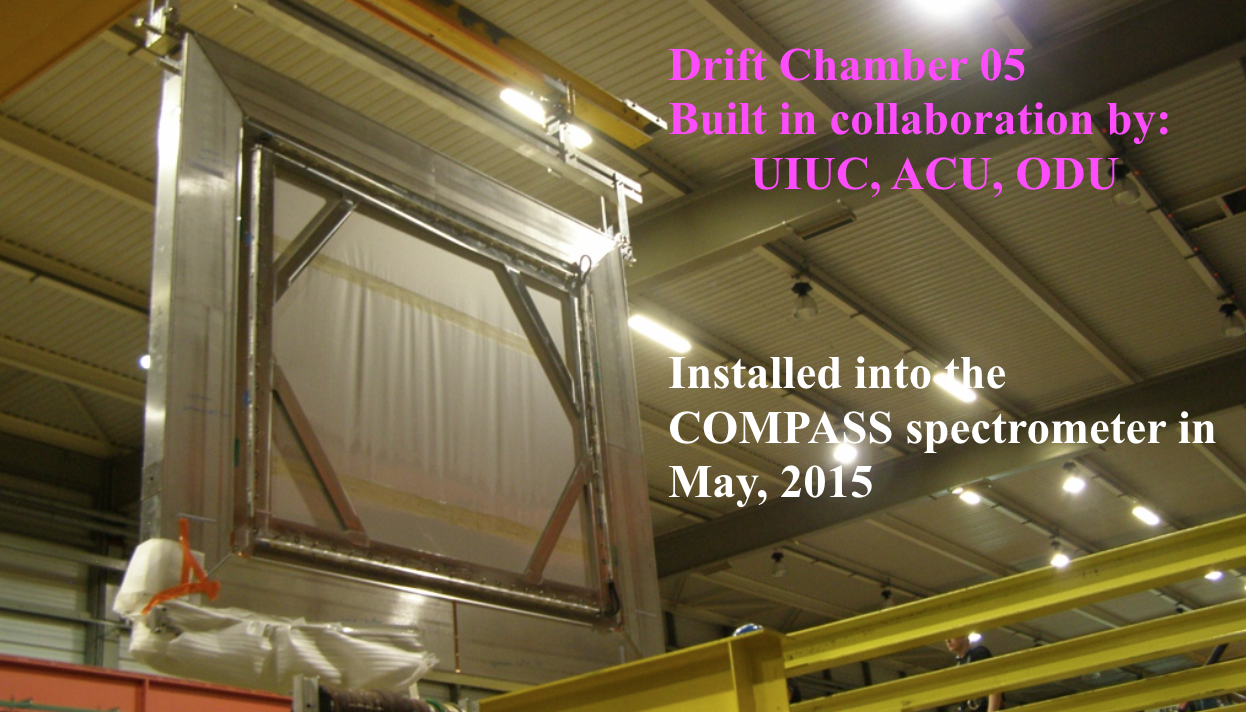
\includegraphics[scale=0.6]{DC05_full}
  \end{figure}
\end{frame}

%\subsection{Motivation}
%\leftskip 0.1in %hanging indent
%\parindent -0.1in
\begin{frame}
  \frametitle{Motivation}
  
  \begin{itemize}
  \item 95\% of high mass Drell-Yan events include a track in LAS.
  \item COMPASS trigger system was setup for a trigger coincidence
    with at least one track in LAS.
  \item Two of the four large area trackers downstream of SM1 (straw
    detectors) in LAS were not performing well.
  \end{itemize}
  
  \begin{columns}
    \column{0.47\textwidth}
    \begin{figure}
      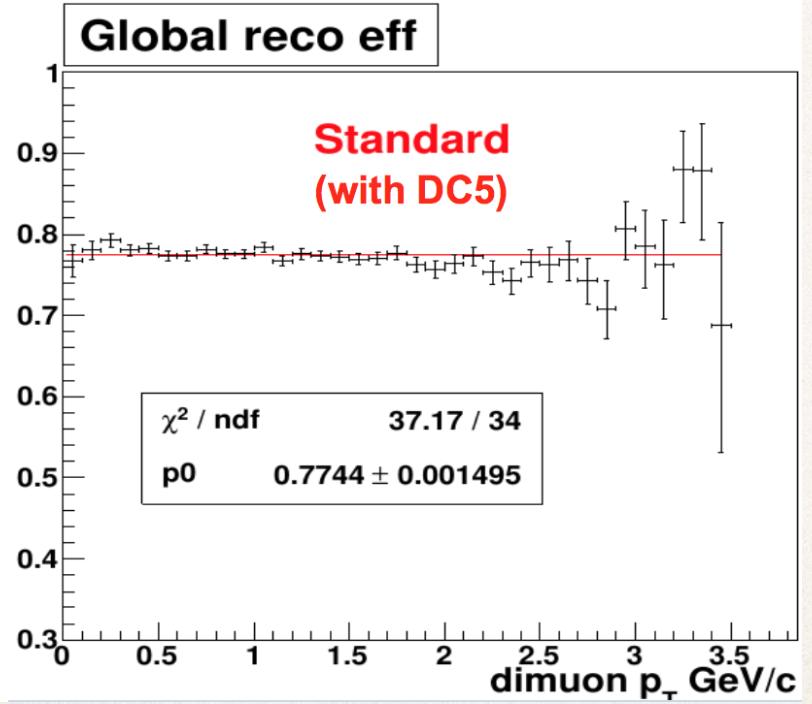
\includegraphics[width=\textwidth]{RecoEff_wDC05}
    \end{figure}
    \column{0.47\textwidth}
    \begin{figure}
      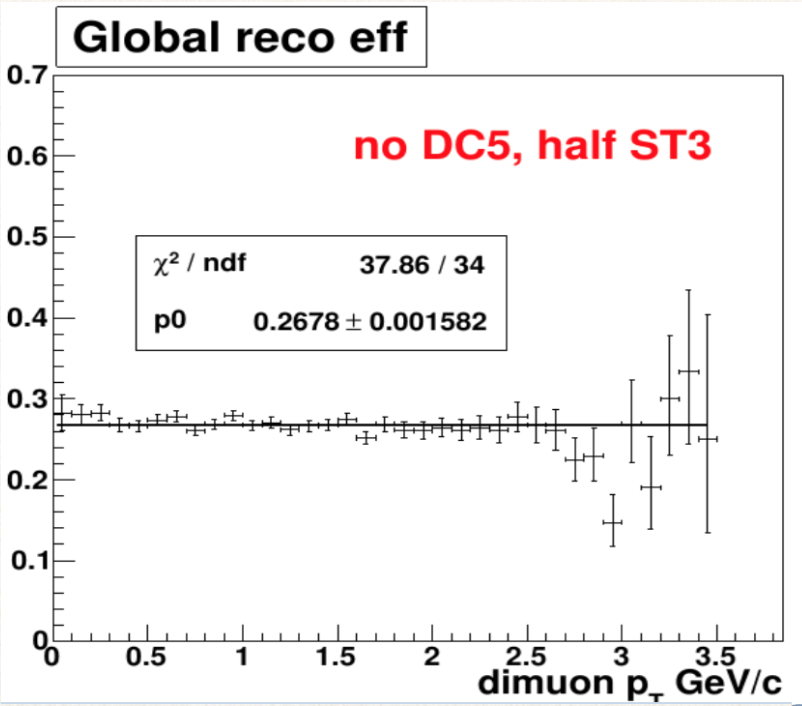
\includegraphics[width=\textwidth]{RecoEff_wOutDC05}
    \end{figure}
  \end{columns}  
  
\end{frame}


\begin{frame}%[label=current]
  \frametitle{DC05 Construction $\qquad \quad \color{red} \mathscr{RH} \text{ contributions to hardware}$}

  \begin{figure}
    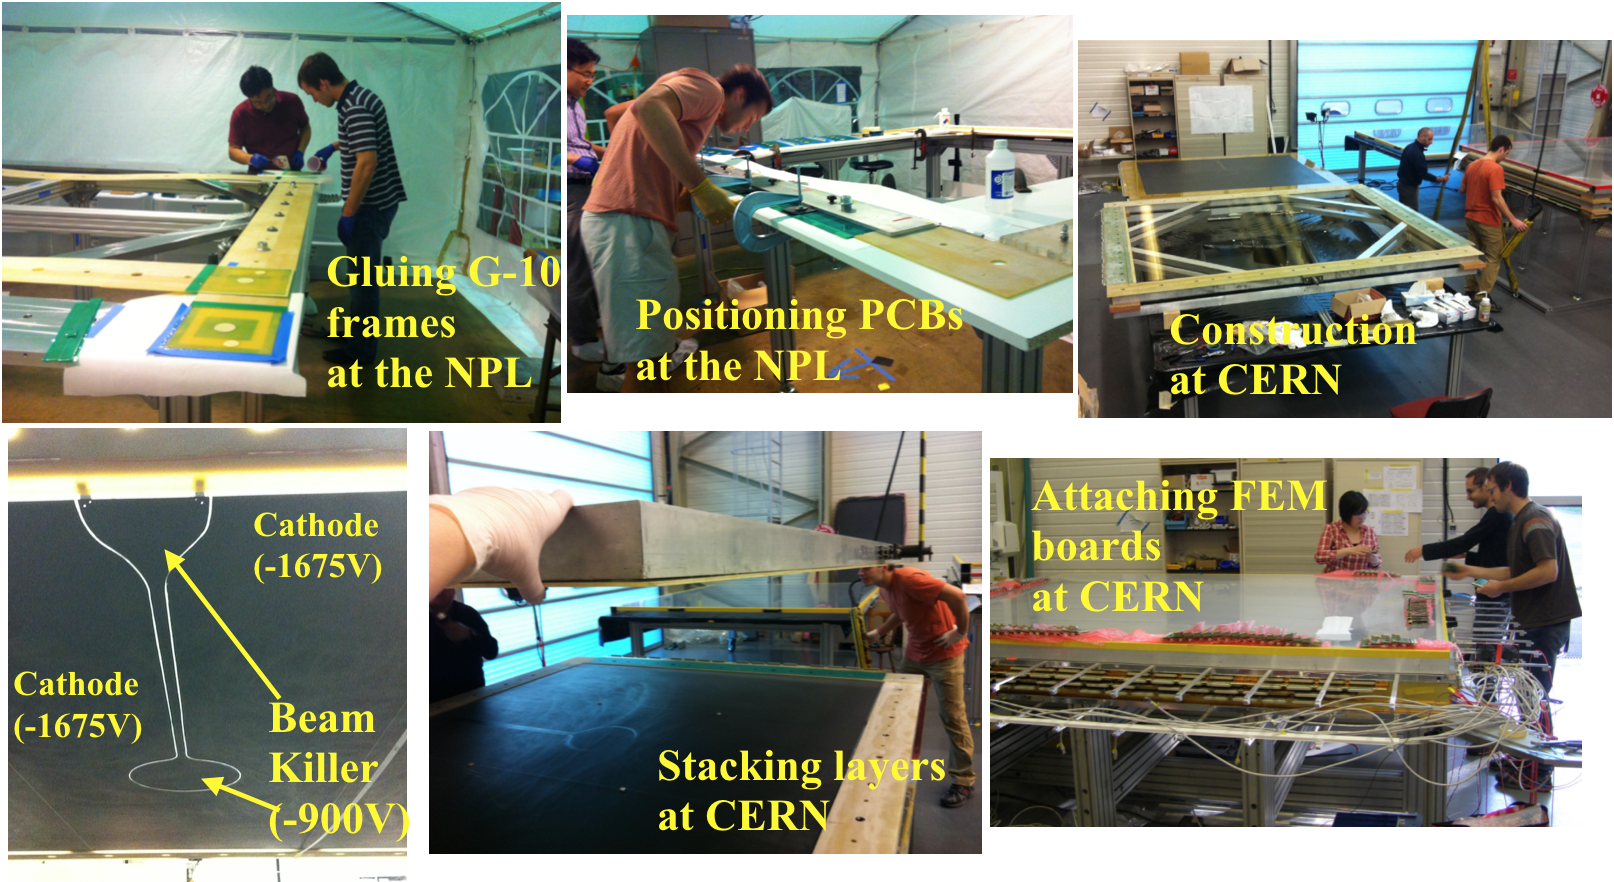
\includegraphics[width=1.05\textwidth]{All_Construction}
  \end{figure}
\end{frame}


\begin{frame}
  \frametitle{Drift Cell (Garfield Simulations)}
  \setlength\abovecaptionskip{-5pt}
  \begin{columns}
    \column{0.47\textwidth}
    \begin{figure}
      \vspace*{-0.4cm}
      \centering
      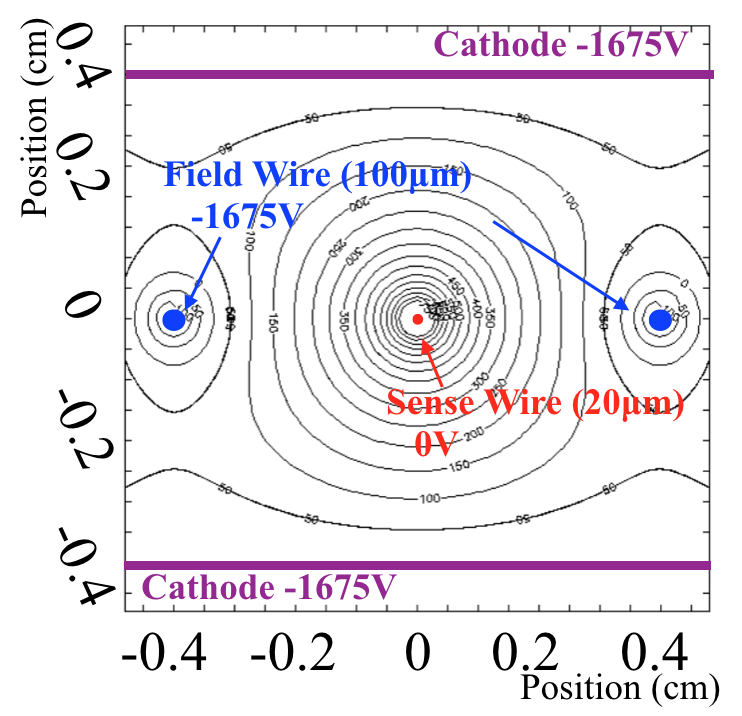
\includegraphics[width=\textwidth]{DriftCell_Pot}
      \caption{Drift cell constant potential lines}
    \end{figure}
    \column{0.47\textwidth}
    \begin{figure}
      \vspace*{-0.4cm}
      \centering
      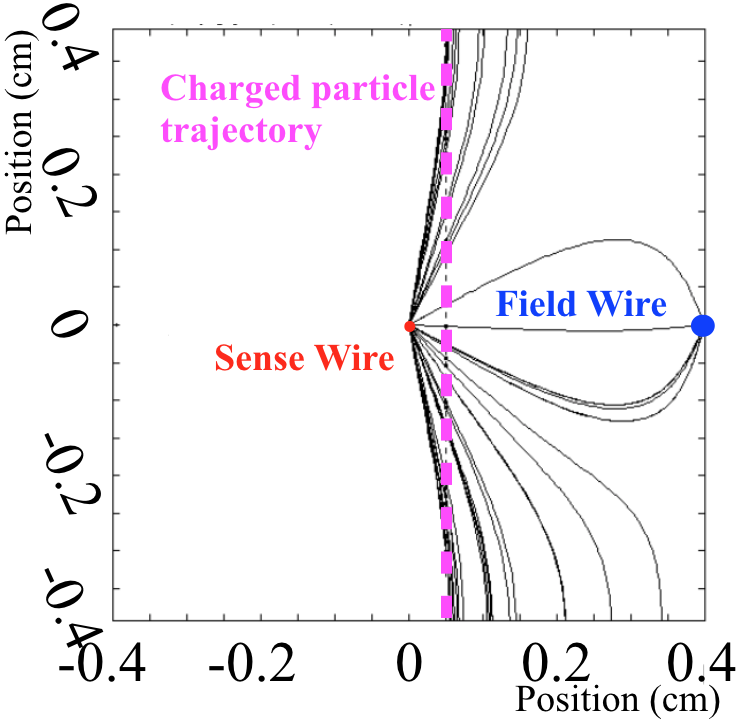
\includegraphics[width=\textwidth]{DriftCell_Particle}
      \caption{Drift cell, electron and ion drift lines}
    \end{figure}
  \end{columns}
  \begin{itemize}
  \item Particle detection occurs per drift cell
  \item Sense wire signals read out by fast front end electronics
  \item DC05 includes 2304 drift cells
  \end{itemize}
\end{frame}


%\subsection{Calibration}
\begin{frame}%[label=current]
  \frametitle{2015 DC05 Calibration $\qquad \color{red} \mathscr{RH} \text{ contributions to analysis}$}

  \begin{figure}
    \centering
    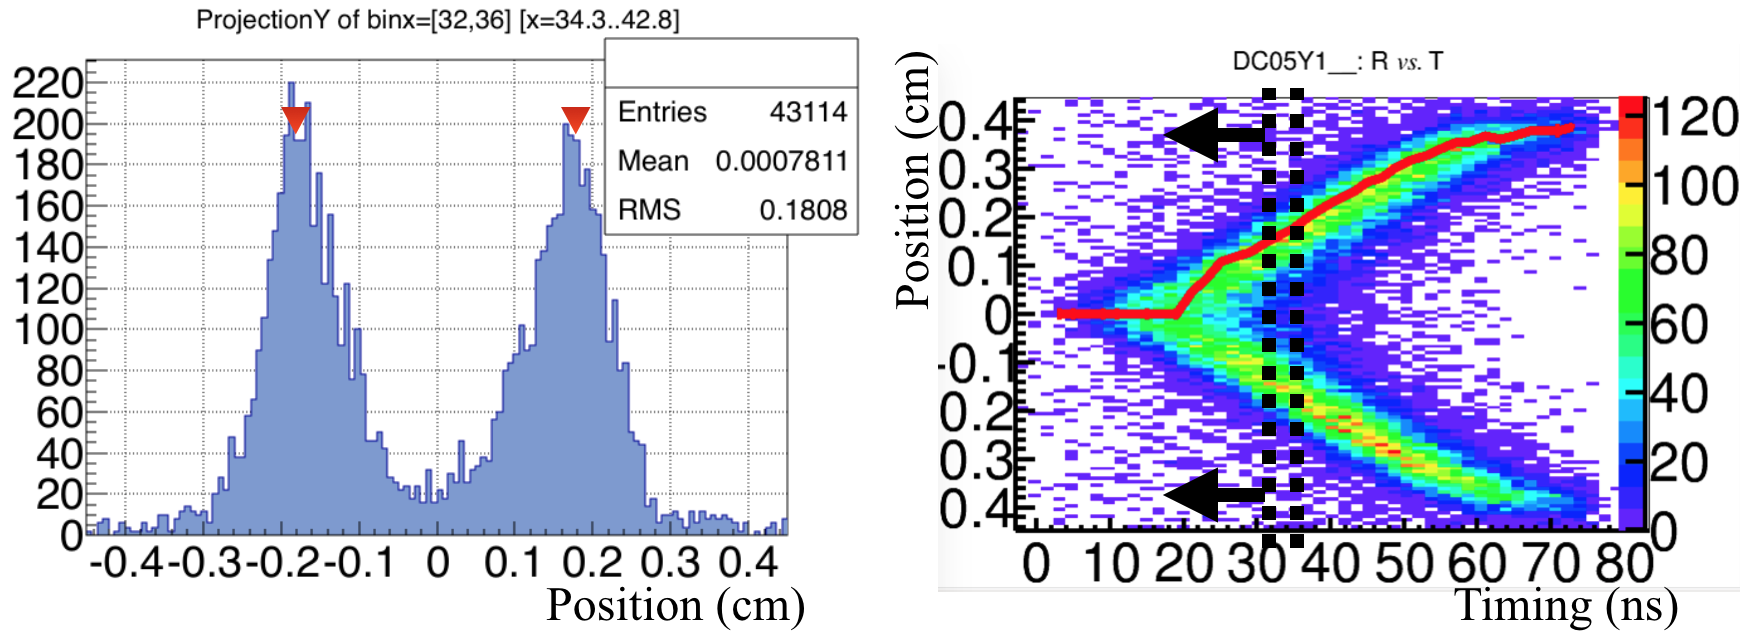
\includegraphics[width=0.9\textwidth]{Calibration}
  \end{figure}
  
  \begin{itemize}
  \item Particle hit position within drift cell
    \begin{itemize}
    \item a function of time after trigger
    \end{itemize}
  \item Drift time calibration improves position resolution
  \item Determined by:
    \begin{itemize}
    \item Excluding view of interest
    \item Reconstruct to find track hit position and timing
      information
    \item Find peaks from y-projections slices
    \end{itemize}
  \end{itemize}
\end{frame}


%\subsection{2015 Performance}
\begin{frame}%[label=current]
  \frametitle{2015 DC05 Efficiency $\qquad \color{red} \mathscr{RH} \text{ contributions to analysis}$}

  \begin{itemize}
  \item Efficiency calculation:
    \begin{itemize}
    \item Reconstructing tracks excluding plane of interest from
      reconstruction
    \item Search for tracks within 1.2mm road of expected hit
      location
    \end{itemize}
  \item 2015 efficiency between 85$\%$ - 90$\%$
  \end{itemize}
  
  \begin{figure}
    \centering
    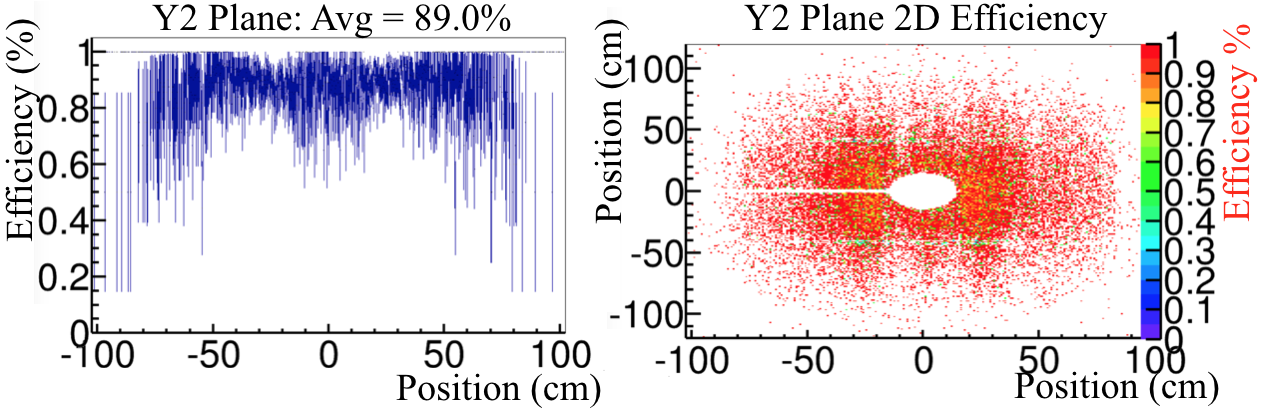
\includegraphics[width=\textwidth]{Efficiency}
    \caption{1D and 2D efficiency plots}
  \end{figure}
\end{frame}



